
\section{Résumé en français}

%%%%%%%%%%%%%%%%%%%%%%%%%%%%%%%%%%%%%%%%%%%%%%%%%%%%%%%%%%%%%%%%%%%%%%%%%%%
\section{Numerical Test Cases}

\subsection{Algorithm and determination of global diffusion coefficient}
\begin{enumerate}
\setlength\itemsep{0pt}
\item Following Winters 1995, first is determined available volume at each depth V(z), then for each time-step build the reference profile by filling V(z) from the bottom up starting with the densest parcels to create $z^*(\rho,t)$ also expressed as $z^*(\mathbf{x},t)$. Study only 2D flows, given the grid sizes Lorenz type of reference profile is not too heavy in computation cost.
\item BPE(t) is computed then its evolution for the volume considered
\item RHS terms of equation \ref{bilanBPEal} (comes from section \ref{section_PE_chap2}) are computed, with some specifities:
\begin{itemize}
\setlength\itemsep{0pt}
\item the term in $dz^*/dt$ is not directly evaluated as such but computed as the sum of terms (1),(2) and (3) of (expression avant equation \label{eq_evolBPE}) for accuracy (the expression in equation \ref{buoyancyzstar} with $\partial \zeta / \partial t$ and Heaviside bigger computation cost too)
\item in the first cases discussed, that are cyclic in both horizontal and vertical direction, advection and diffusion through the vertical boundaries is possible and those terms are computed to have the complete balance between right hand side and left hand side.
\item $\kappa_h$ and $\kappa_v$ are the unknown variable of the problem. considered homogeneous for the volume considered, and in most cases consider $\kappa_h=\kappa_v=\kappa$ (isotropic), because impossibility except when know there is no diffusion in one direction to differentiate between the two contributions.
\item In this case $\kappa_{eff}$ expressed as equation \ref{eq_kappaEff}
\end{itemize}
\item The aim of this chapter is to evaluate the efficiency of this method and where it needs to be further refined.
\item First use a simple advection - harmonic explicit diffusion model with constant volume. In a second time apply to CROCO to several simple test cases to end with the realistic case of simulation SimRef of chapter \ref{chapGBR2D}.
\end{enumerate}


\begin{subequations}
  \begin{alignat}{2}
  \displaystyle 
 	&\frac{d E_b}{d t} &&= \quad \underbrace{g\int_x \int_{-1}^0 \rho h \frac{d z^*}{d t}\bigg\rvert_{xs} \ dx ds}_{\phi_{\zeta}}\\
 & && \quad \underbrace{- g\bigg[ \int_{-1}^0 \rho h z^* u \ ds\bigg]_{x} - g\bigg[ \int_x\rho z^* v_s \ dx\bigg]_0^1}_{F_A} \\
 & && \quad \underbrace{+ g  \kappa \ \bigg[ \int_{-1}^0 h z^*  \frac{\partial \rho}{\partial x}\bigg\rvert_{ts} \ ds \bigg]_{x}
 + g \kappa \ \bigg[ \int_x z^* \frac{1}{h} \frac{\partial \rho}{\partial s}\bigg\rvert_{tx} \ dx \bigg]_0^1 }_{\kappa F_D}\\
 & && \quad \underbrace{- g \kappa \int_x \int_{-1}^0 h  \frac{d z^*}{d \rho} \frac{\partial \rho}{\partial x}\bigg\rvert_{ts}^2 \ dx ds 
 - g \kappa \int_x \int_{-1}^0 \frac{1}{h} \frac{d z^*}{d \rho} \frac{\partial \rho}{\partial s}\bigg\rvert_{tx}^2 \ dx ds}_{\kappa \phi_D}
\end{alignat}
\label{bilanBPEal}
\end{subequations}

An instantaneous evaluation of diffusivity is :
\begin{equation}
\kappa_{eff} = \frac{\frac{dE_b}{dt}-(\phi_{\zeta}+F_A)}{F_D+\phi_D}
\label{eq_kappaEff}
\end{equation}


\subsection{NUMLAB experiment}
2D Simple advection-harmonic diffusion code giving evolution of a quantity $\psi$, cyclic in each direction. 
\begin{equation}
\frac{\partial \psi}{\partial t} = -u\frac{\partial \psi}{\partial x} - w\frac{\partial \psi}{\partial z} + \kappa_{exp}^x \frac{\partial^2 \Psi}{\partial x^2} + \kappa_{exp}^z \frac{\partial^2 \psi}{\partial z^2}
\end{equation}
with $\kappa_{exp}^{x,z}$ an explicit diffusion coefficient that can be given.

No change in volume so $\phi_{\zeta}$ integrate to zero for all Numlab cases. No vertical velocity, $v_s=0$, so the second term of both $F_a$ is zero.

Initial tracer field is either $\psi(x)=cos(2\pi x/L_x)$ or $\psi(x,z)=Re(e^{i2\pi x/L_x}e^{i 2 \pi z/L_z})$. 


\subsubsection{Local diffusion case}

\begin{figure}[h!]
\centering
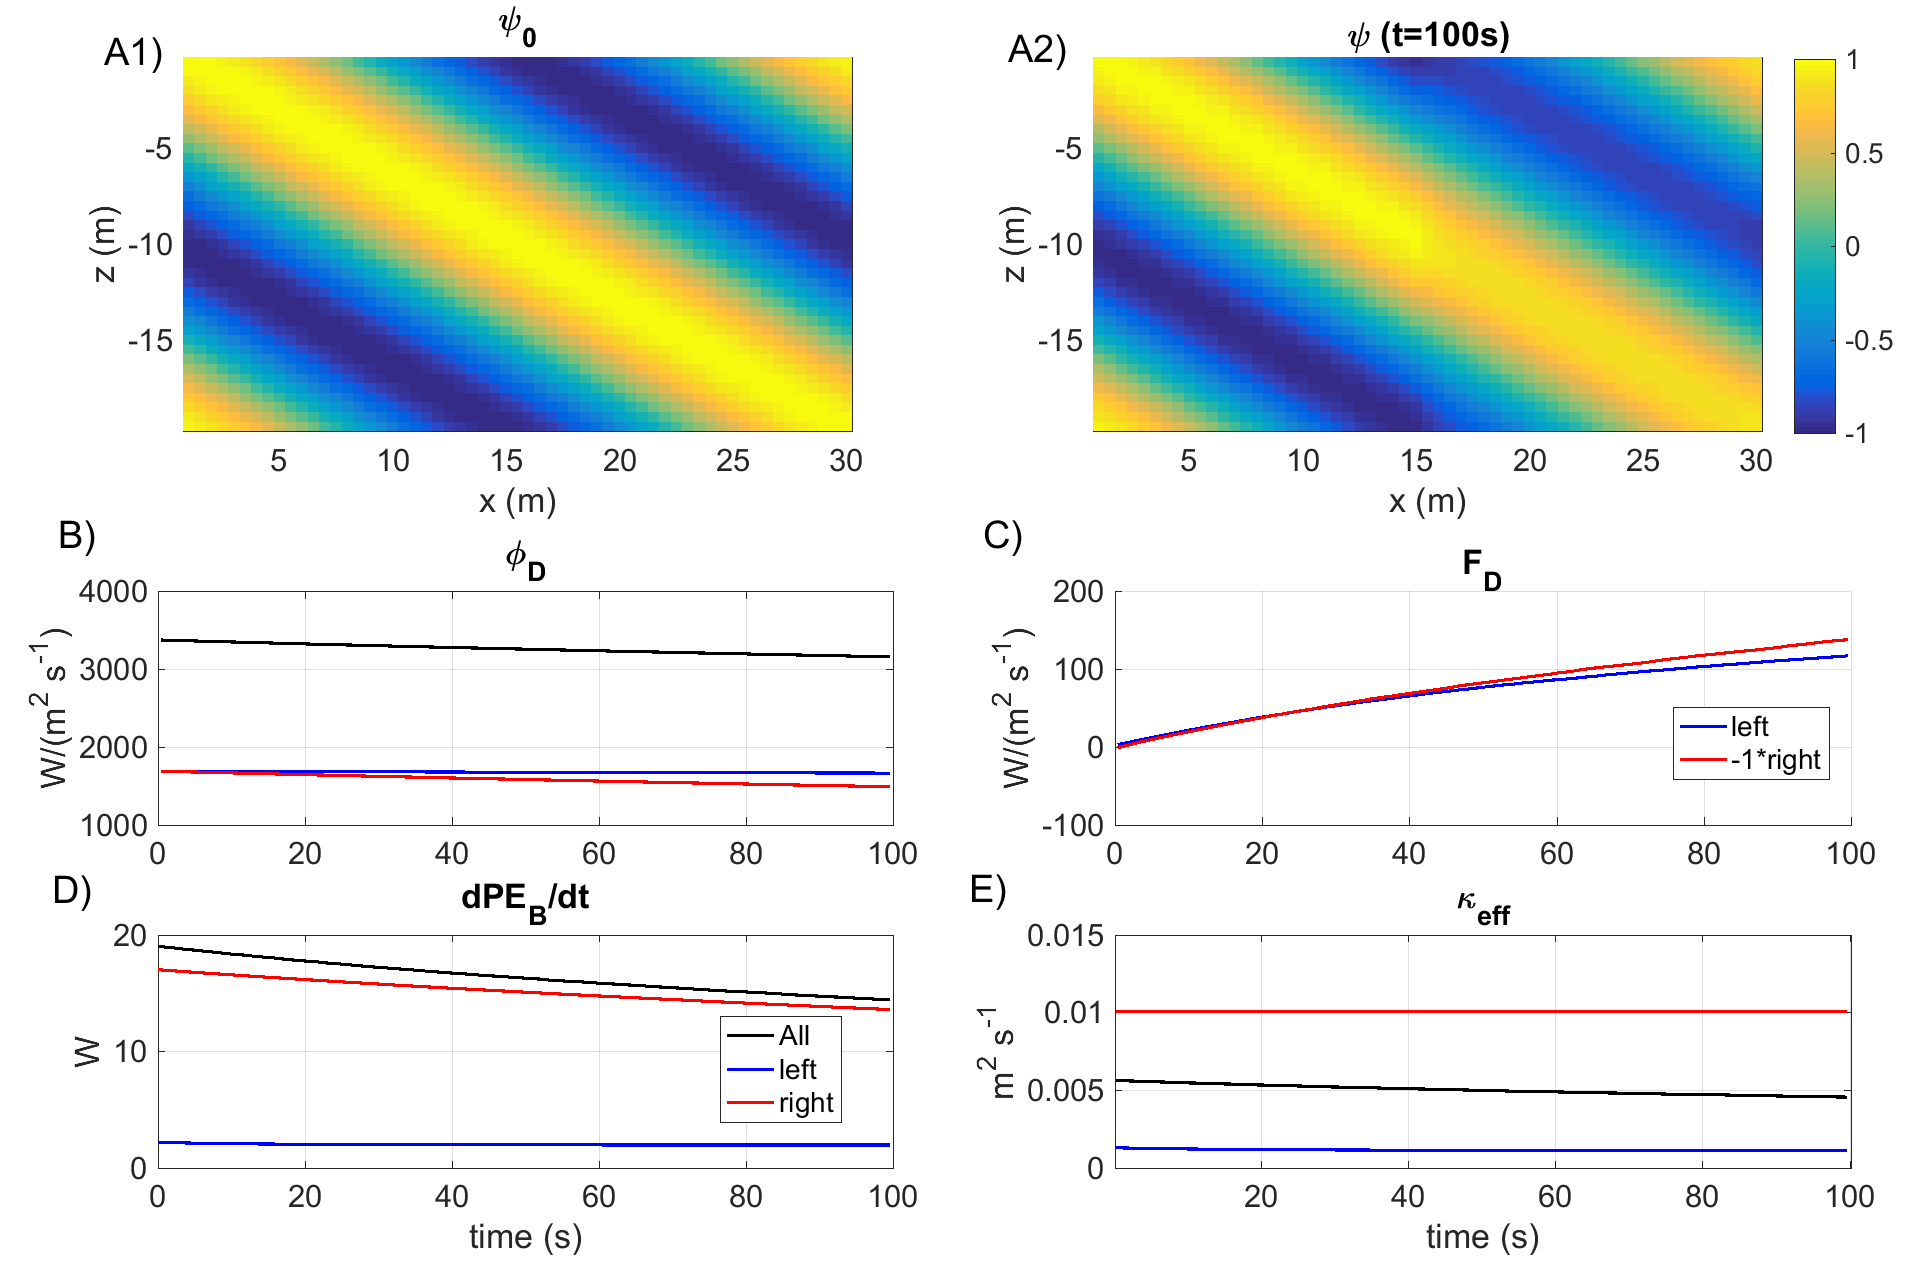
\includegraphics[width=1\textwidth]{./CHAP_BPE/AGBPE_numlab2.png}
\caption{(c) is \ref{bilanBPEal}e... Ajouter champ initial?}
\label{fig2numlab}
\end{figure}

%Initial tracer field same as in fig \ref{fig1numlab}.
\begin{itemize}
\item Figure \ref{fig2numlab}. $dx=0.5$ m, $dz=0.5$ m, $L_x=30$ m, $L_z=20$ m, $dt=0.1s$. $\kappa_{exp}^x=\kappa_{exp}^z=\kappa_{exp}$ and $u=0$, no advection. RK3 timestepping scheme.
\item For x$<$15 m, $\kappa_{exp} = 10^{-3}$, otherwise $\kappa_{exp} = 10^{-2}$ m$^2$/s.
\item compute $\kappa_{eff}$ either for each half domain or the whole domain. Three different reference profiles $z^*$ : $z^*_{left}$,$z^*_{right}$,$z^*_{all}$, this means that the sum of for exemple $\phi_D^{left}+\phi_D^{right}$ is nbot equal to the same term computed on the whole domain, in the same vein the the diffusive fluxes do not cancel each other.
\item When $\kappa_{eff}$ evaluated on each half domain, find the good values $\kappa_{eff}=\kappa_{exp}$. When on whole domain, start at average value but decreases. It will tend to the lowest value since in the right half, gradient of $\psi$ will be deteriorated quicker, hence the term of the integrand is smaller and the higher value of the gradient of $\psi$ in the left half will... (je n'arrive pas à formuler : l'évolution pilotée par là où le coef est le plus bas une fois que les gradients à droite sont résorbés)
\item only able to differentiate for $\kappa(x)$. If diffusion coefficient was made to vary along the vertical direction, in the same way that when evaluate $\kappa_{eff}$ for the whole domain, integrates all contributions to the change in $z^*$ in the water column
\end{itemize}

\subsubsection{Implicit diffusion case : IMP}

\begin{itemize}
\item $dx=0.5$ m, $dz=0.5$ m, $L_x=30$ m, $L_z=20$ m, $dt=0.1s$ same as previously, but this time $U=0.1m/s$, and advection scheme either RK3-UP1 or RK3-UP3. Want to evaluate implicit diffusion $\kappa_{imp}$ of each scheme and compare to what the development of the discrete equation gives as formulation. 
\end{itemize}


\underline{\textit{2nd order scheme : UP1}}
\begin{figure}[h!]
\centering
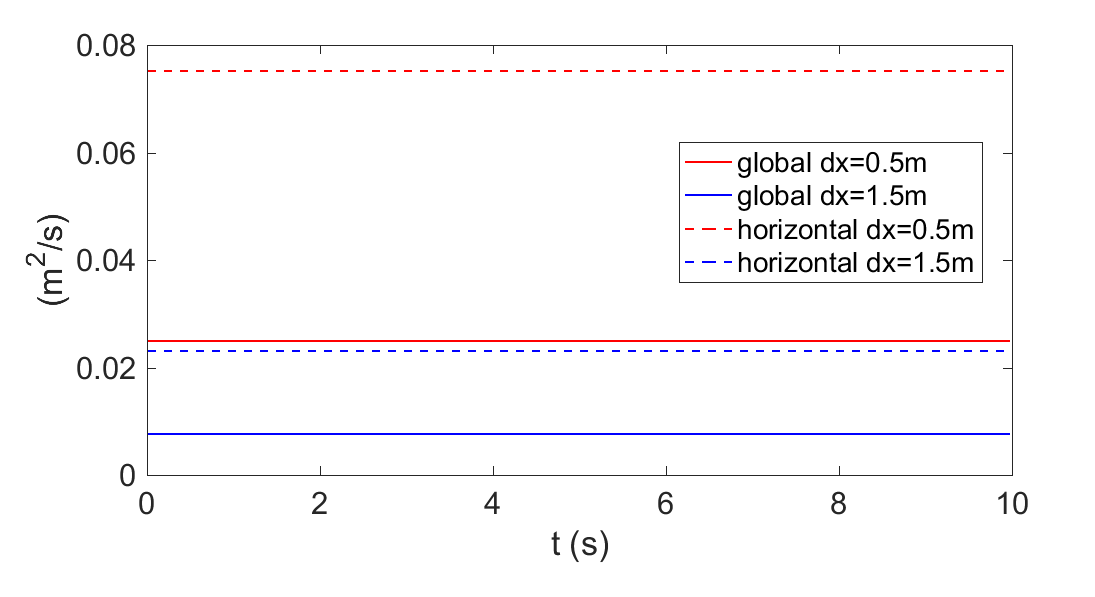
\includegraphics[width=0.5\textwidth]{./CHAP_BPE/AGBPE_numlab3.png}
\caption{Diffusion coefficient for implicit diffusion case RK3-UP1. Either assume $\kappa_z=\kappa_x$(horizontal) or that $\kappa_z=0$ (global)\color{red}(Il faudra que je repasse sur ecrtaines figures)\color{black}}
\label{fig3numlab}
\end{figure}

Initial field same as previous case. RK3-UP1 scheme with horizontal velocity. No explicit harmonic diffusion ($\kappa_{exp}=0$). Development of discrete advection equation gives formulation of an implicit diffusion coefficient $\kappa_{h,i}=\frac{1}{2}U \Delta x$ 
\begin{equation}
U \frac{\partial \psi}{\partial x} +\frac{\partial \psi}{\partial t} = \frac{1}{2} U \Delta x  \frac{\partial^2 \psi}{\partial x^2} + o(\frac{\partial^3 \psi}{\partial x^3})
\end{equation}
$dx=0.5$ m then $dx=1.5$ m, gives values of $\kappa_{h,i}$ of 0.025m$^2$/s and 0.075m$^2$/s

Figure \ref{fig3numlab}. Find the good value $\kappa_{eff}=\kappa_{imp}$ if don't take into account term of vertical diffusion, only along current. Otherwise the value of $\kappa_{eff}$ found is lesser since it is taken as applied to contribution for both horizontal and vertical diffusion.

\underline{\textit{4th order scheme : UP3}}

Initial tracer field is $\psi(x,t=0)=cos(2\pi x/L_x)$ (see figure (\noparref{fig5numlab}.a)), so that the analitical solution of advection-diffusion problem is : $\psi(x,t)=e^{-\kappa k_x^2 t}cos(k(x-Ut))$ with $k_x=2\pi/L_x$

RK3-UP3 advection scheme with horizontal velocity. Expending the discrete scheme gives 4th order diffusion.
\begin{equation}
U \frac{\partial \psi}{\partial x} +\frac{\partial \psi}{\partial t} = \underbrace{\frac{1}{120}(5 C^3-10) U \Delta x^3}_{k_4}  \frac{\partial^4 \psi}{\partial x^4} + o(\frac{\partial^5 \psi}{\partial x^5})
\end{equation}
where C is the advection Courant number, here $C=2 . 10^{-2}$. Fourth order coefficient is $k_4=-1.10^{-3} m^4/s$. However, the BPE analysis give an implicit diffusion in form of second order with coefficient $k_2=\kappa_{eff}$.

\begin{itemize}
\item A serie of exeperiment is made where in addition to the implicit diffusion cause by the advection scheme, add explicit harmonic diffusion. The effective coefficient found by BPE analysis is $\kappa_{eff} = \kappa_{exp} + \kappa_{imp}$.
\item See in figure \ref{fig5numlab}.b (case for which $\kappa_{exp}=0$ ) that have high-frequency oscillations of non-negligible relative amplitude.\color{red}(correspond temps d'advection d'une cellule??? à vérifier (ou vient calcul des termes du bilan pas en RK3?))\color{black}. The value of $\kappa_{eff}$ found is averaged over the 200s of the simulation, find value of $\approx 4.65.10^{-5} m^2/s$. In the same way $\kappa_{eff}$ is computed for serie of simulation with explicit coefficient non zero and averaged, $\kappa_{imp}$ is taken as this average minus the explicit value that was initially given. Always find the same value of  $\approx 4.65.10^{-5} m^2/s$.
\item This value is for harmonic diffusion, in figure (\noparref{fig5numlab}.c), compare on a random point of simulation with $\kappa_{exp}=0$ the evolution of $k_4 \frac{\partial^4 \psi}{\partial x^4}$ and $k_2 \frac{\partial^2 \psi}{\partial x^2}$ with $k_2=4.65.10^{-5} m^2/s$, the evolution is close but not exaclty equal.
\end{itemize}



\begin{table}[h!]
\centering
\begin{tabular}{|l|l|l|l|l|l|l|l|l|l|l|}
\hline
$\kappa_{exp}$ & $-10^{-4}$ &$-4.65.10^{-5}$ & $-10^{-5}$& $0$& $10^{-5}$& $10^{-4}$\\
\hline
$\kappa_{eff}$ & $-5.35.10^{-5}$ &$3.5.10^{-8}$ & $3.65.10^{-5}$& $4.65.10^{-5}$& $5.65.10^{-5}$& $14.65.10^{-5}$\\
\hline
$\kappa_{imp}$&\multicolumn{6}{c|}{$4.65.10^{-5}$}\\
\hline
\end{tabular}
\caption{Explicit coefficient given to simulation, effective coefficient computed from BPE analysis and implicit coefficient by deducting one from the other}
\end{table}

\begin{figure}[h!]
\centering
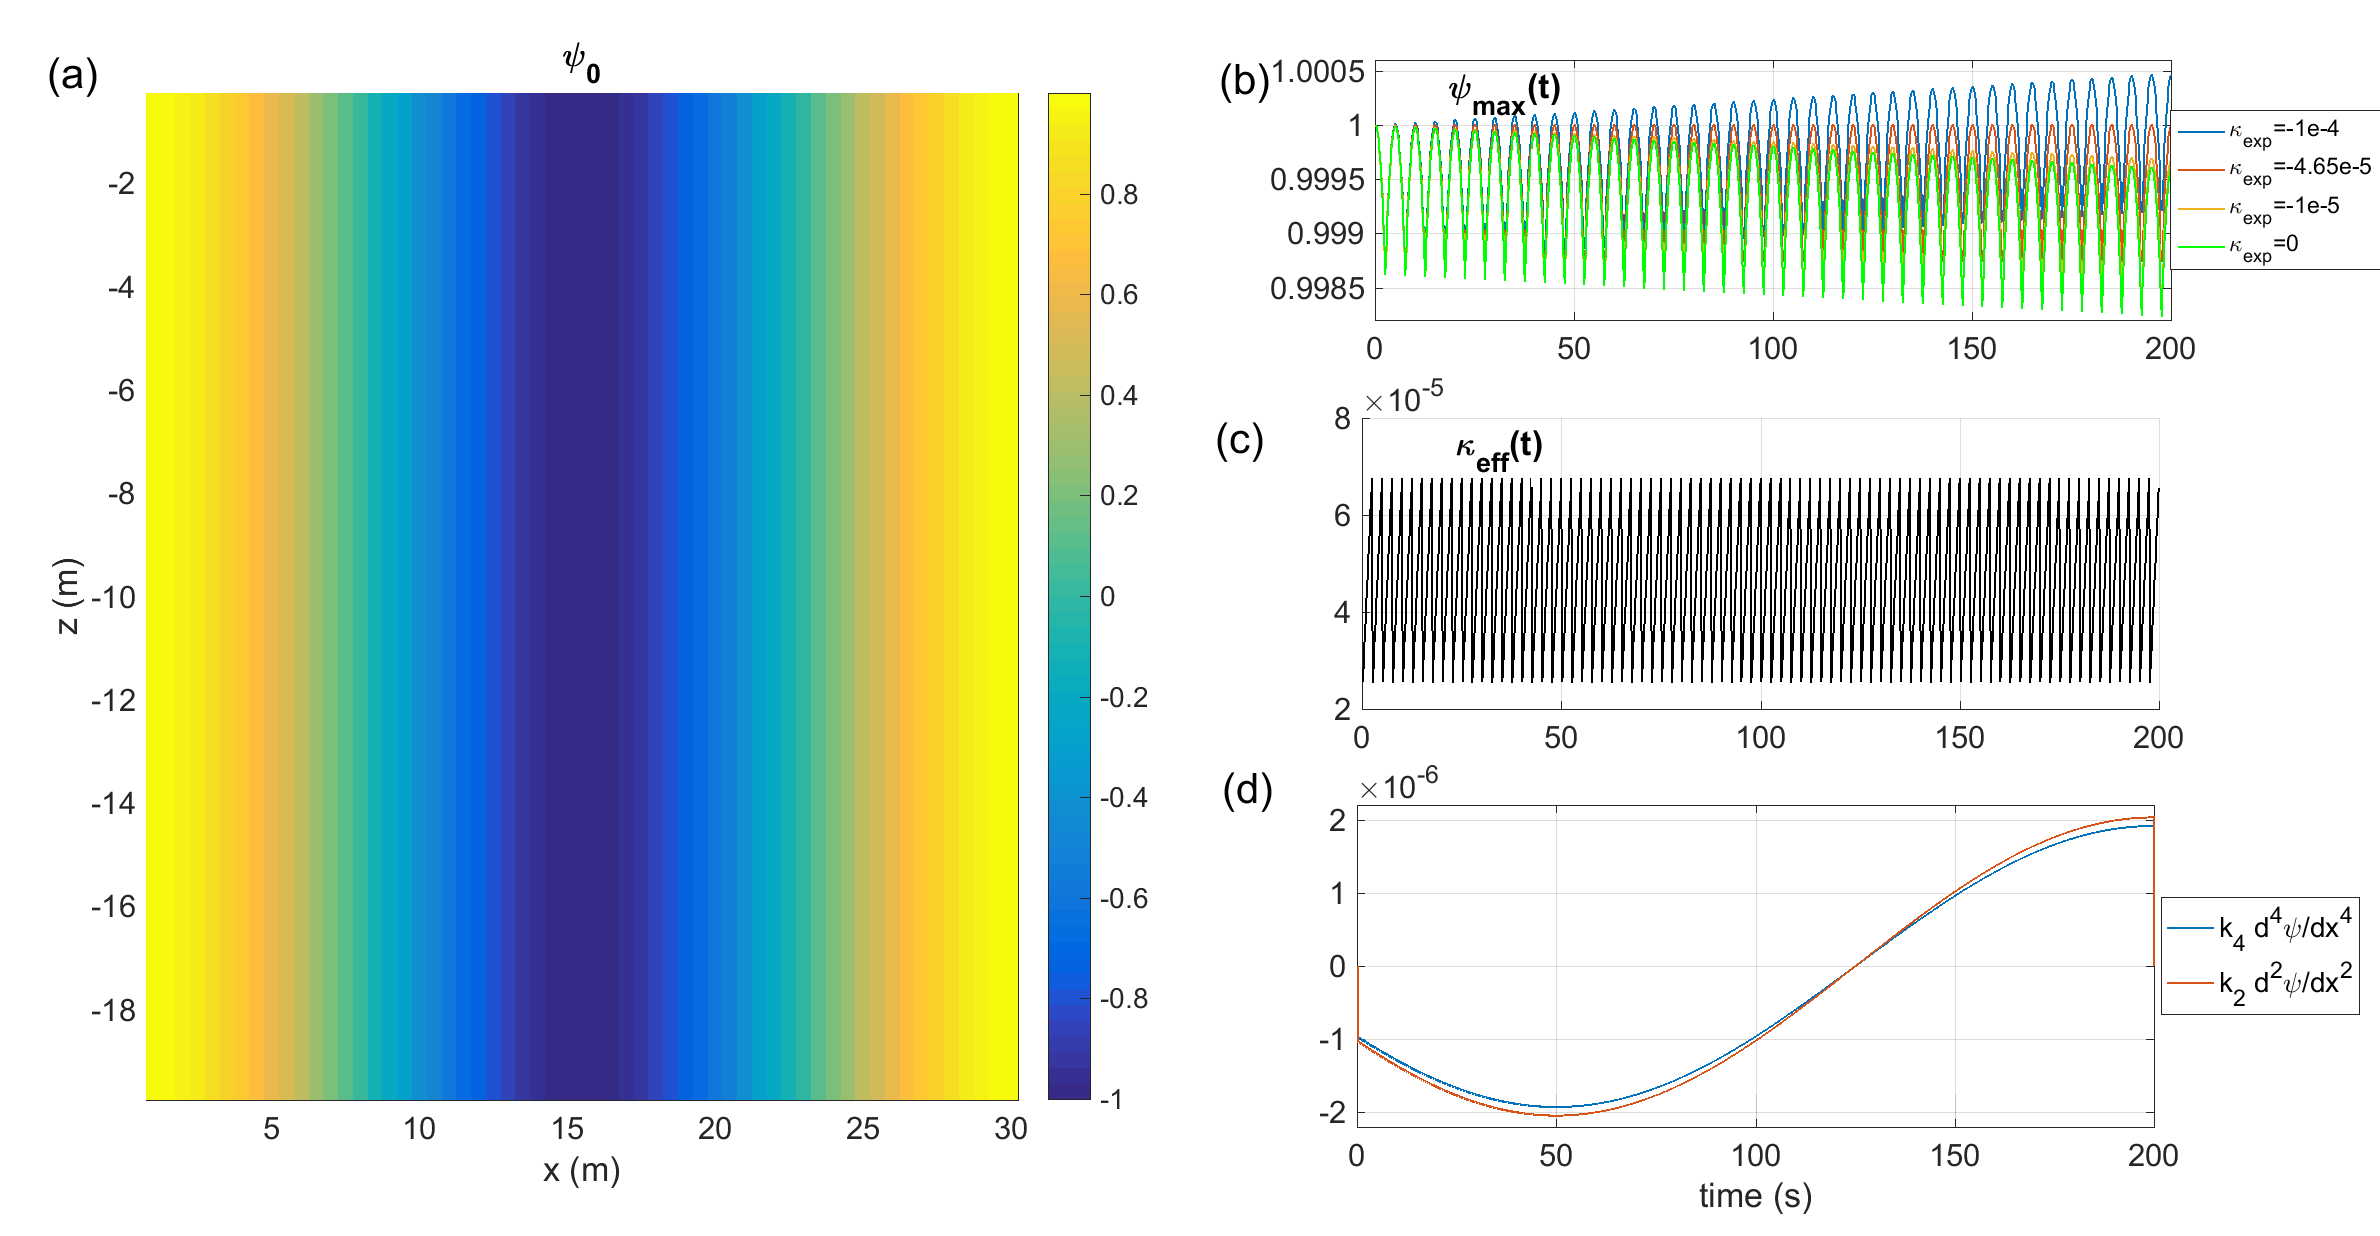
\includegraphics[width=1\textwidth]{./CHAP_BPE/AGBPE_numlab5.png}
\caption{(a) initial field  (b) maximum value of $\psi$ in the field  (c) value of $\kappa{eff}$ by instantaneous balance for case with no explicit diffusion $\kappa{exp}=0$ (d) comparison fourth order and second order formulation\color{red}(Enlever figure avec les max de $\psi$)\color{black}}
\label{fig5numlab}
\end{figure}


\subsubsection{Diffusion and advection timescales}
\begin{figure}[h!]
\centering
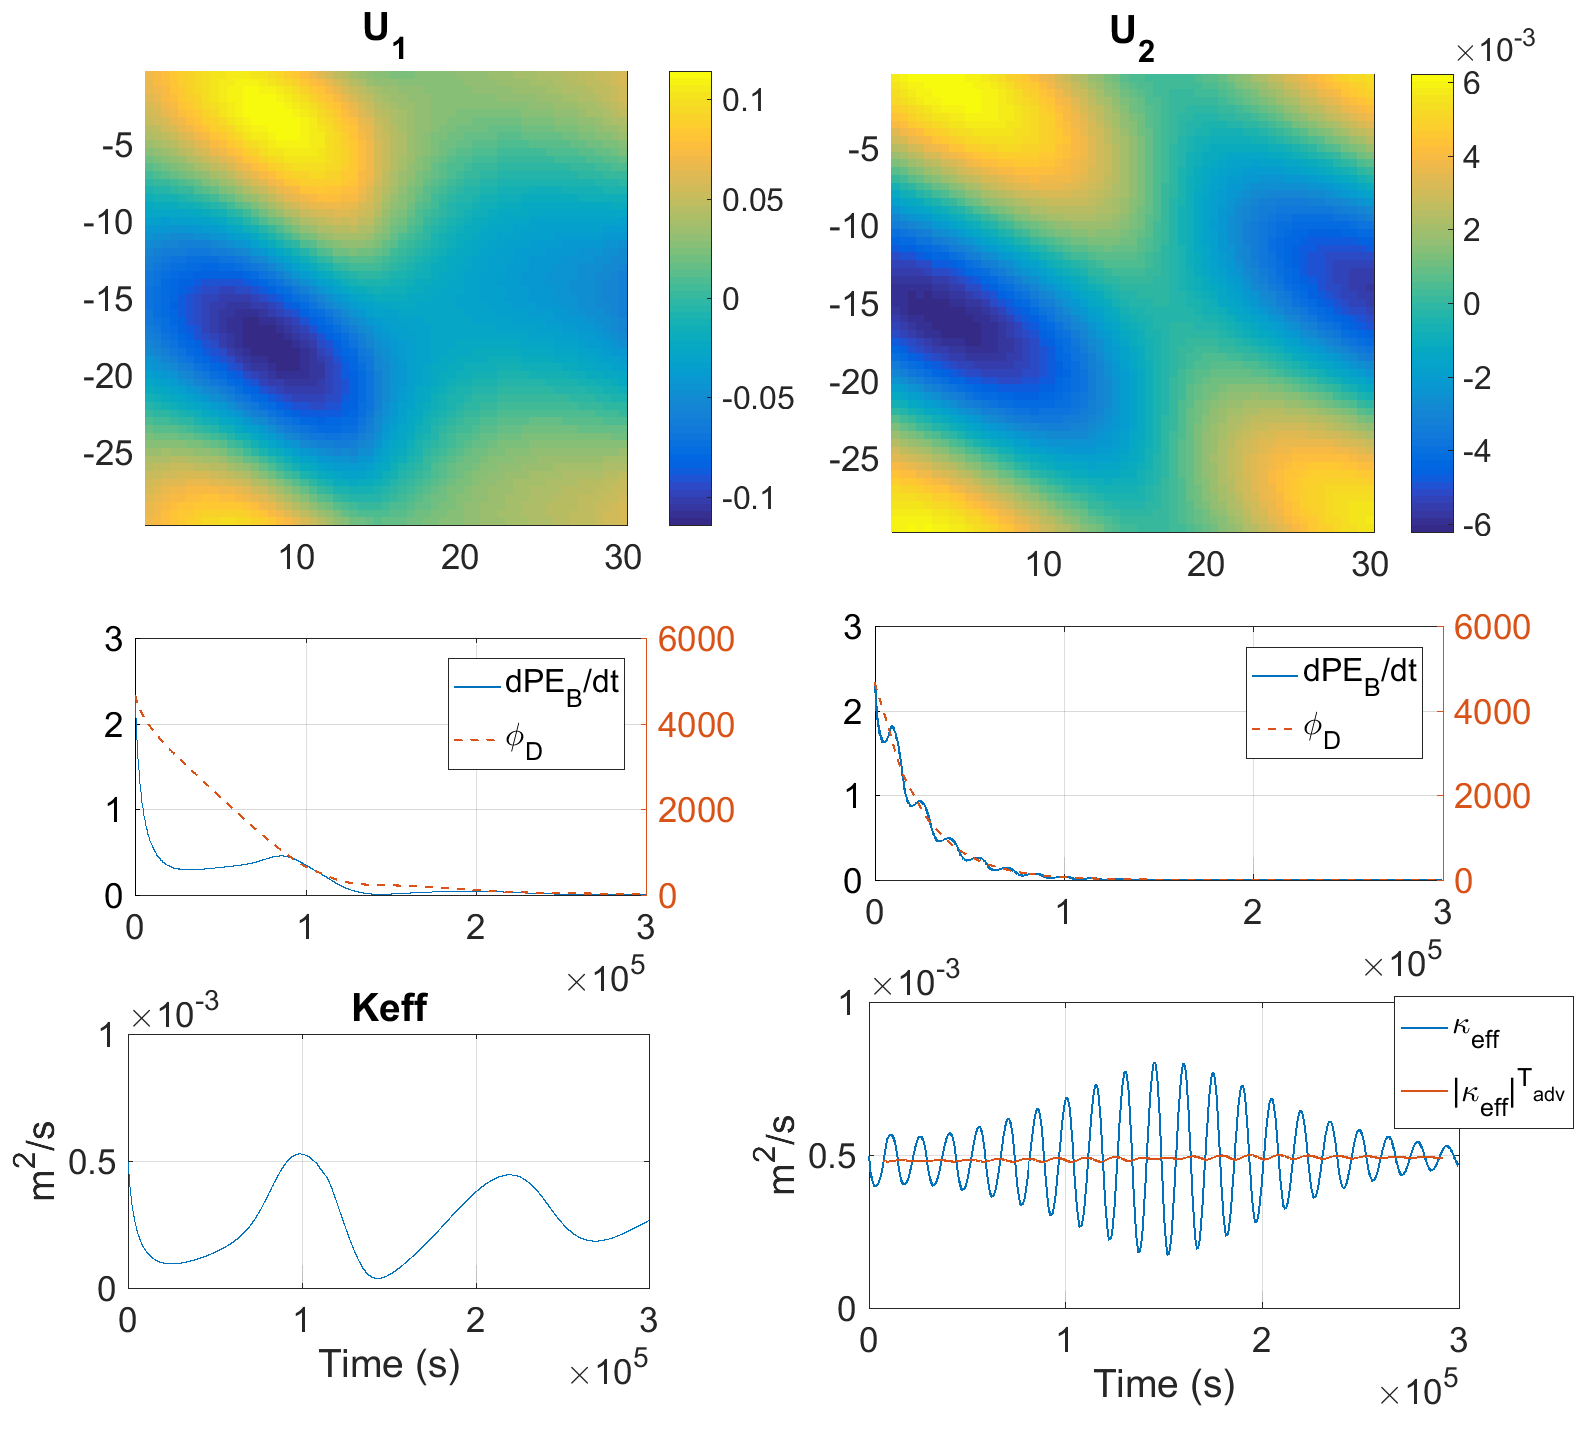
\includegraphics[width=1\textwidth]{./CHAP_BPE/Fig_numlab_advdiff3.png}
\caption{ }
\label{fig4numlab}
\end{figure}
\begin{itemize}
\item RK3-C2 scheme (no implicit diffusion). $\Delta x = \Delta z = 0.5m$, $L = H = 30m$, $dt=10s$
\item $\kappa(x)$ avec $\kappa = 10^{-5} \ m^2/s$ for left half of domain and $\kappa = 10^{-3} \ m^2/s$ for right half. 
\item Horizontal advection, two cases, either $U_1=2 \ 10^{-4} m/s $ or $U_2=2 \ 10^{-3} m/s $
\item Can estimate timescales for advection, $T_{adv}=L_{adv}/U$, and for diffusion $T_{\kappa}=L_{\kappa}^2/{\kappa}$. With L the characteristic length/size of the structure affected by each process. Here diffusion on each half domain so $L_{\kappa}=15m$. Advection same value for all domain, $L_{adv}=30m$.
\item So $T_{\kappa}^{left}=2.25 \ 10^7 \ s$, $T_{\kappa}^{right}=2.25 \ 10^5 \ s$, and depending on the value of $U$ $T_{adv}^{U_1}=1.5 \ 10^5 \ s$ or $T_{adv}^{U_2}=1.5 \ 10^4 \ s$
\item $T_{adv}^{U_2}<<T_{adv}^{U_1}<T_{\kappa}^{right}<<T_{\kappa}^{left}$
\item Figure \ref{fig4numlab} . See appearance of the field after t=$1.35 \ 10^5 \ s$ for each advection value. With $U_1$ (left) $t<T_{adv}^{U_1}$ the displacement of the structure is minimal compared to the initial field, but $t$ is close to $T_{\kappa}^{right}$ and see that there structure is far more dissipated than on the left. With $U_2$ however, $t>>T_{adv}^{U_2}$ several advection periods have occured and field is symetric but overall if look at values of colorbar have had more dissipation (faire apparaitre les gradients)
\item  Look at the $\kappa_{eff}$ computed for each velocity for the whole domain. the median of the two values of diffusivity in the domain is $5 \ 10^{-4} \ m^2/s$. This value is initially taken in case $U_1$, $T_{\kappa}^{right}$ and $T_{adv}^{U_1}$ are close, see oscillation but center below the median value and not regular%but after $t=3.86 \ 10^4 s$ , reach a minimum of $\kappa_{eff}=3.24 \ 10^{-5} m^2/s$. This value then increases again slowly then stabilizes at $\kappa_{eff}=2.2 \ 10^{-4} \ m^2/s$ after $t=2.785 \ 10^5 s$ approx half $T_{adv}^{U_1}$ at this point all original fluid parcels have been advected through the high dissipation area.
\item case $U_2$, see centered around the median value but with oscillations HF at $T_{adv}^{U_2}$ and a modulation at lower frequency (dissipation one? ça à l'air d'être le bon ordre de grandeur)
\item When compute on each half domain, find the expected values with lesser oscillations at the timescales discussed above. But on the whole domain, lagrangian evolution of gradients (ie following advection through areas of varying dissipation) can make interpretation of $\kappa_{eff}$ if advection and diffusion timescales are close. 
\end{itemize}



%%%%%%%%%%%%%%%%%%%%%%%%%%%%%%%%%%%%%%%%%%%%%
\subsection{CROCO experiments : TANK}

Now apply determination of $\kappa_{eff}$ to numerical cases Based on TANK experiment (ref?), adapted to have stratification. Evolution of the density tracer field, through the complete system of equation for ocean CROCO. Closed domain, 2D. No initial velocity. 

\subsubsection{Linear vertical stratification and free surface : role of $dz*/dt$}

\begin{figure}[h!]
\centering
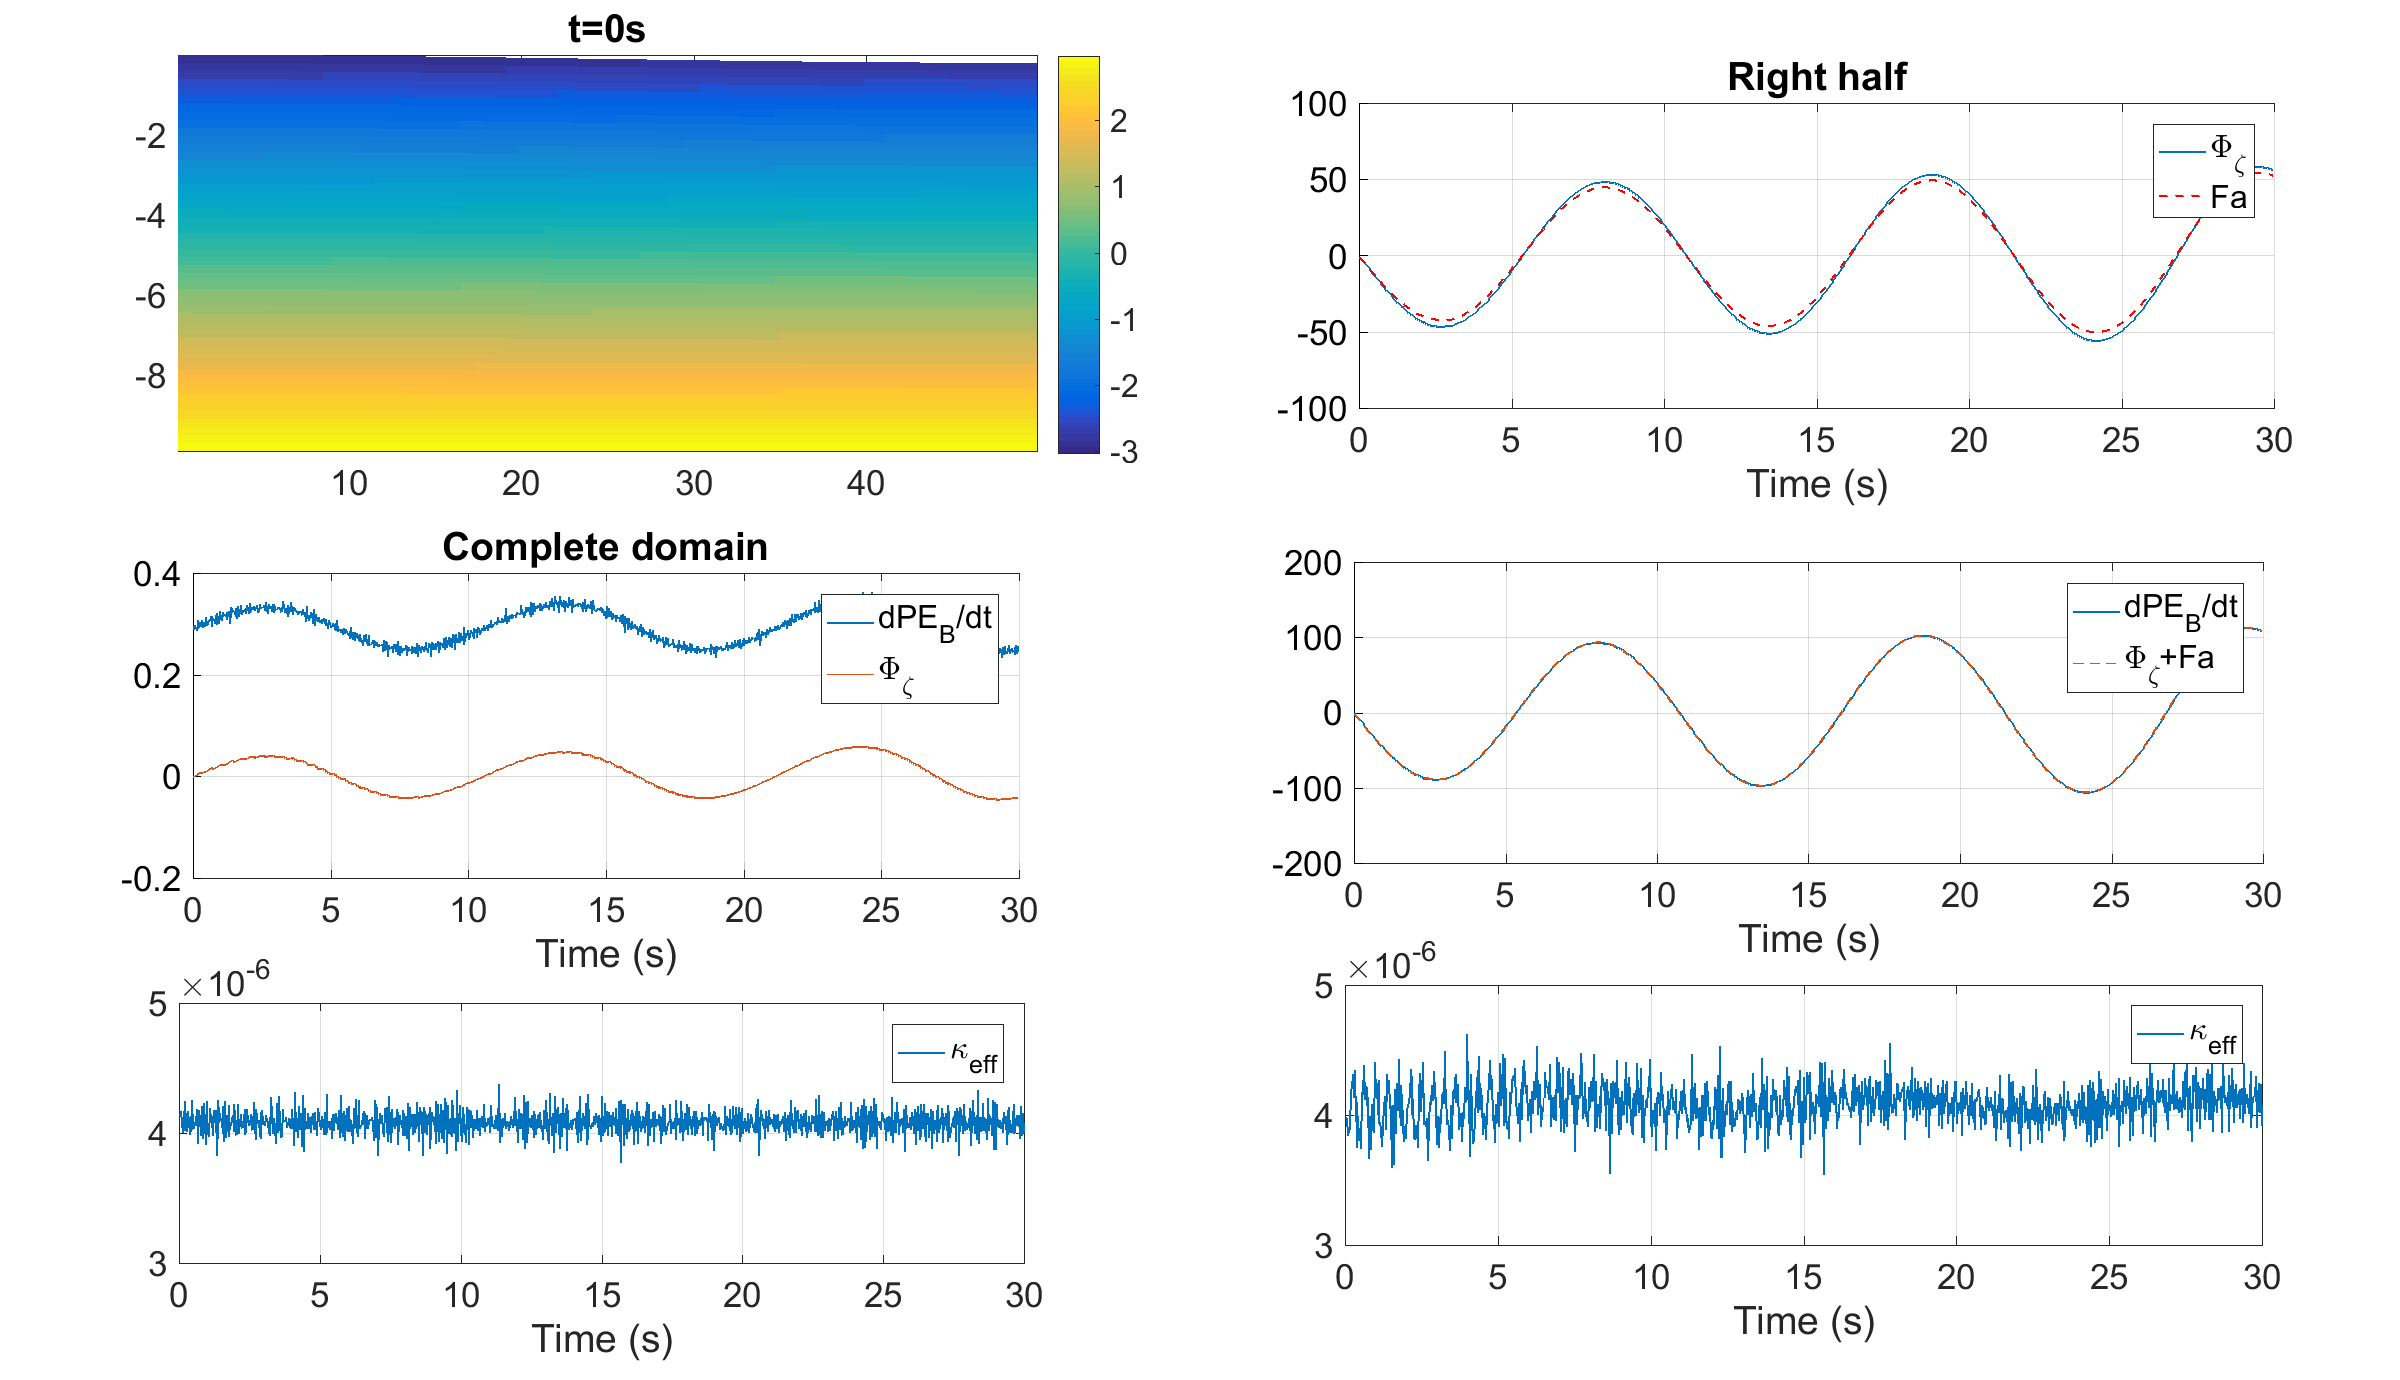
\includegraphics[width=1\textwidth]{./CHAP_BPE/Fig_TANK_linS.png}
\caption{Cas strat lineaire}
\label{figClin}
\end{figure}

\begin{itemize}
\item Movement comes from evolution of initially non-flat free surface. Initial linear stratification $\rho(z)$ (ie, constant N) see figure (\noparref{figClin}.A). $\rho_0=1043 kg/m^3$
\item L$=$50m, H$=$10m, dx$=$0.2m$\approx$dz, amplitude oscillation initiale de la surface libre de 2mm. Explicit diffusion coefficient put at $10^{-4}$m$^2$/s. 
\item fig \ref{figClin} : initial field and computation of $\Phi_{\zeta}$ and other terms. Computation on the whole domain, see amplitude of oscillation of $dPE_B/dt$ is due to $\Phi_{\zeta}$.
\item $u=\sqrt(gH)=9.9 m/s$ the speed of surface waves, so a timescale associated with an anomaly of the free surafce travelling from one border to the order $T_{\zeta}=L/u=5s$. See that the oscillations of $dPE_b/dt$ are in $2*T_{\zeta}$.
\item If make computation on a half domain $\Phi_{\zeta}$ is of the same amplitude as $F_a$ the advective fluxes. All terms are bigger.
\item find $\kappa_{eff}$ of the explicit value that was given. Without taking into account $\Phi_{\zeta}$ would have leftover oscillations.
\end{itemize}

\subsubsection{Pycnocline and free surface}

\begin{figure}[h!]
\centering
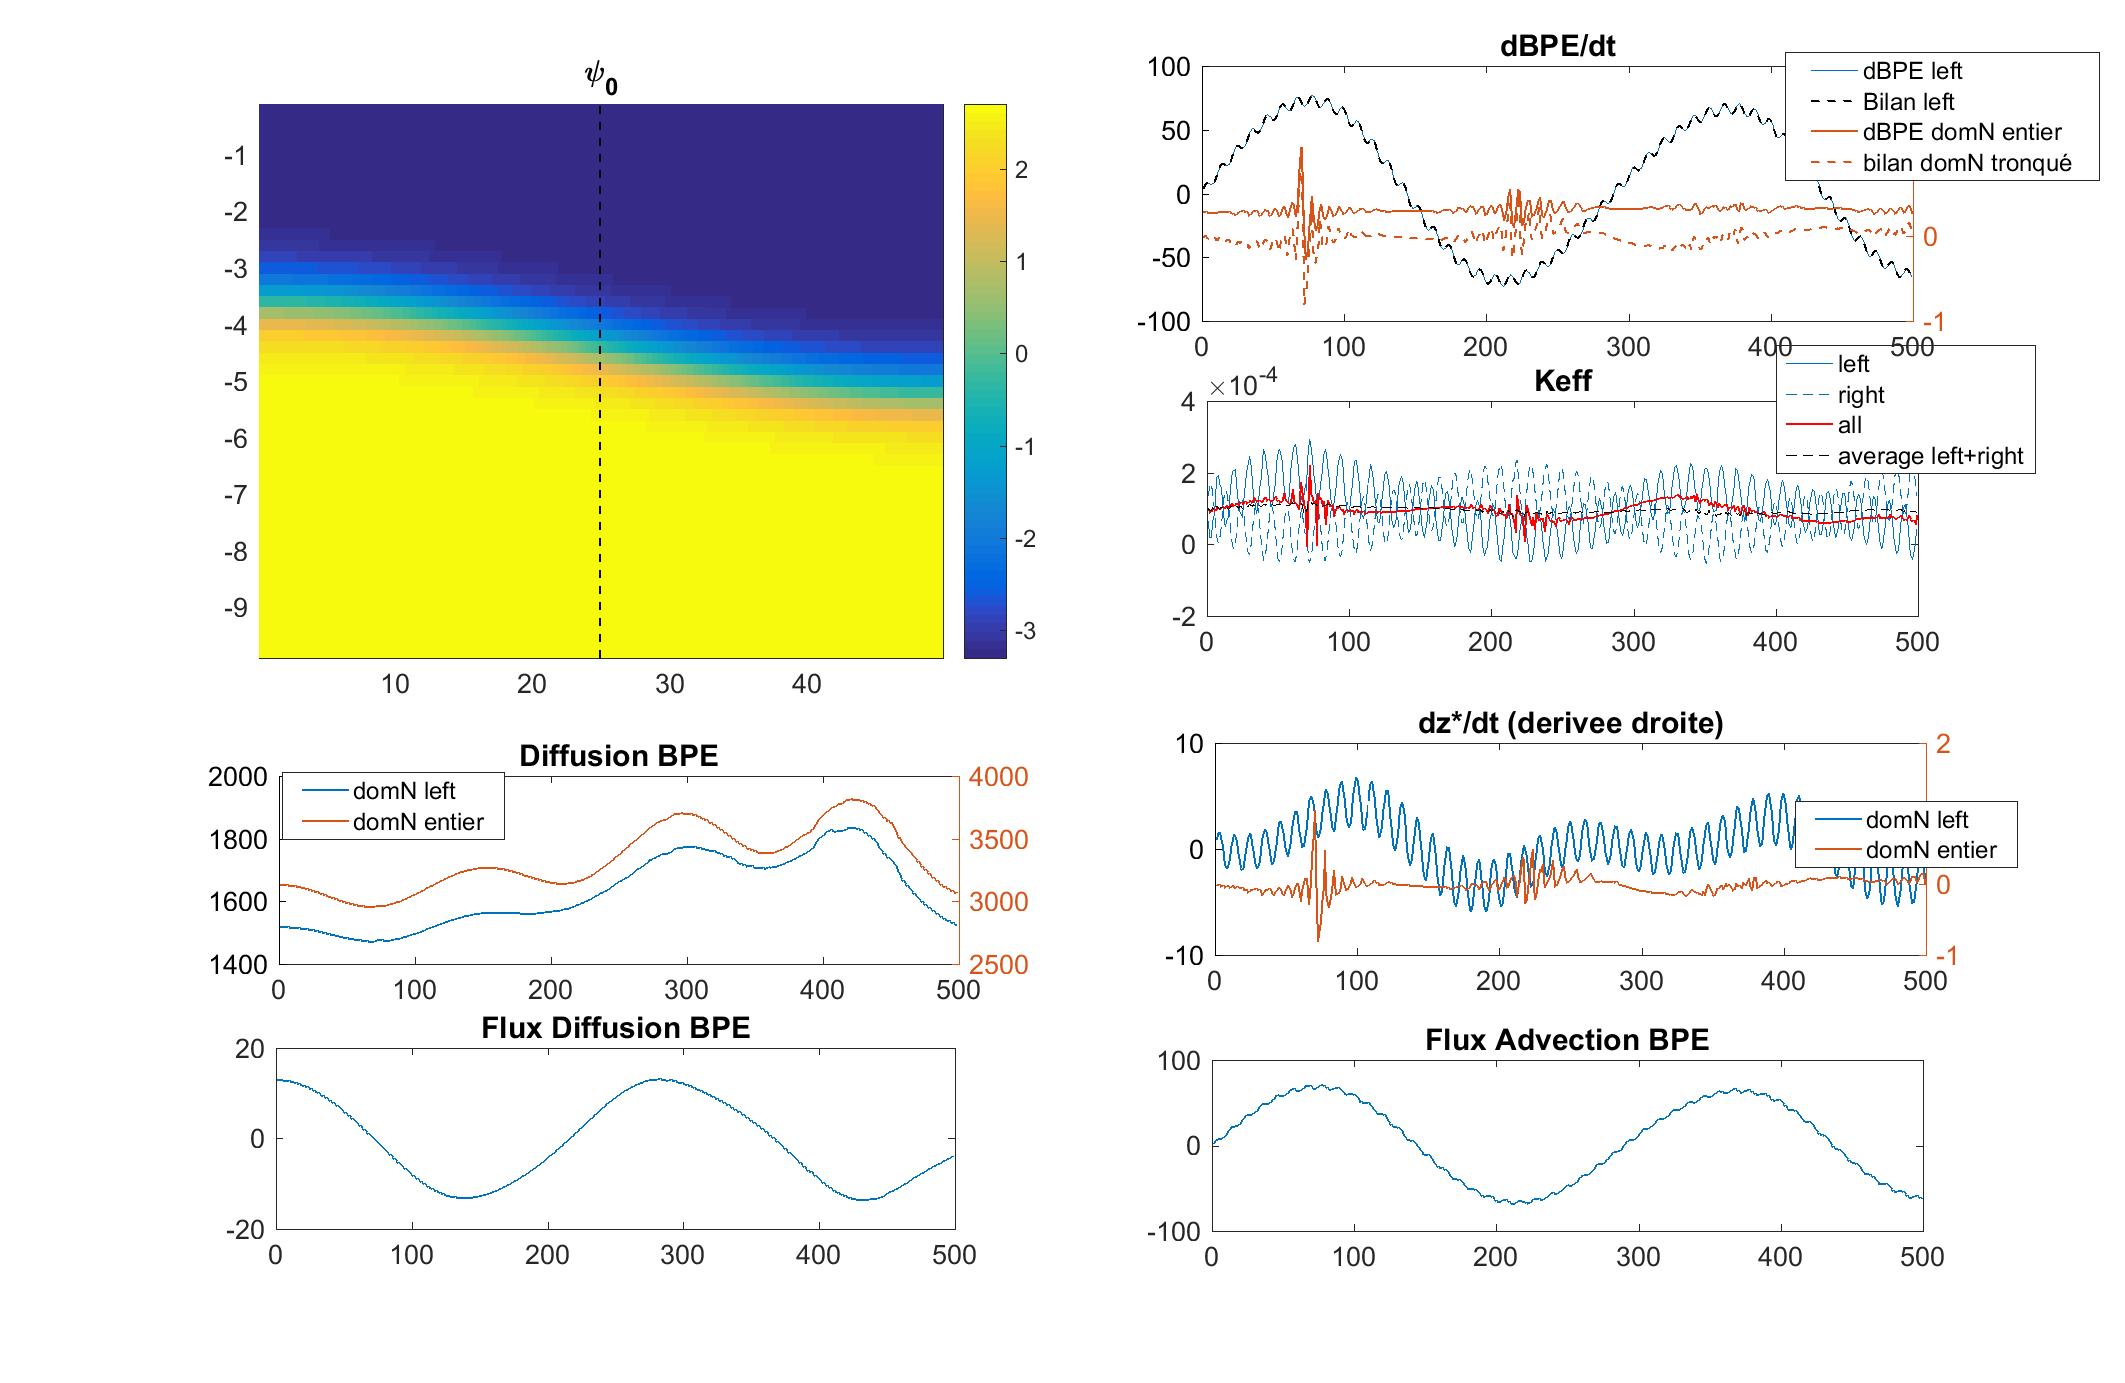
\includegraphics[width=1\textwidth]{./CHAP_BPE/AGBPE_numlab7.png}
\caption{TANK Pycnocline case.bottom row : advection and diffusion flux in regard to the left domain(as discussed in numlab part, do not cancel with fluxes computed for the right half)\color{red}half domain : mettre que un des côtés (?) et faire des moyennes glissante.... Mettre que la figure champ initial et dBPE et Keff\color{black}}
\label{figCpsin}
\end{figure}

\begin{itemize}
\item dx$=$dz$=$0.2m, L$=$50m, H$=$10m. Explicit coefficient put at $10^{-4}$m$^2$/s. \color{red}$\rho_0=$\color{black}
\item Speed surface waves $\sqrt(gH)=5m/s$ and $T_{\zeta}=5s$
\item interfacial wave $\sqrt(g'h_1h_2/H)=0.33m/s$ and $T_{\eta}=150s$
\item Initial stratification in figure \ref{figCpsin}.A not balance (sinusoidal shape), movement of interface.
\item If filter the high-frequency free-surface contribution in each half domain, see increase in BPE (positive value of dBPE) when the depth of the interface increases, and respectively BPE will decrease as the interface gets shallower.
\item figure \ref{figCpsin} see that the timescale associated with free surface appears for computation on half domains. Otherwise timescale associated with the interface for half domain and also for all the domain. See for all domain a signal (pics a $t=80s$)
\item note that oscillations in half domain can sometime give a $\kappa_{eff}$ of negative value ( à expliquer... car le prend homogene et isotrope?)
\end{itemize}



\subsubsection{Pycnocline, free surface and bottom bathymetry}
\begin{figure}[h!]
%\begin{subfigure}{.5\textwidth}
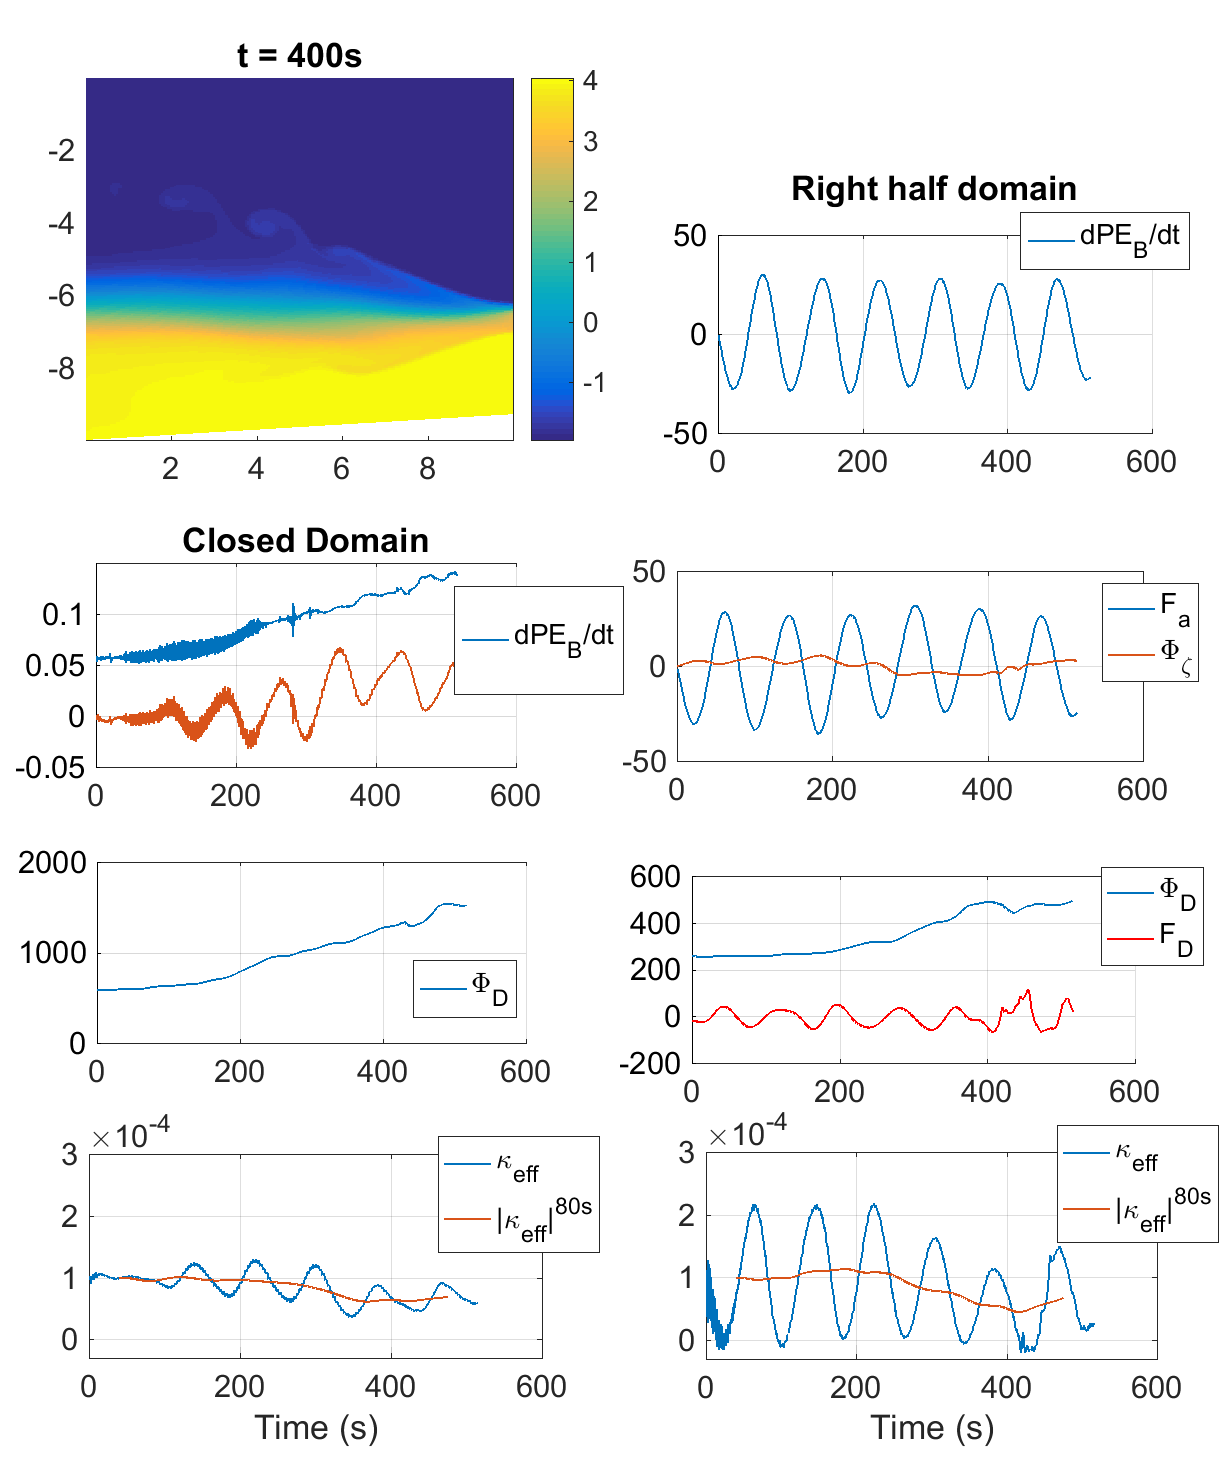
\includegraphics[width=1.\textwidth]{./CHAP_BPE/Fig_TANK_pycbath.png}
%\caption{Closed domain}
%\label{figCkh}
%\end{subfigure}
\caption{Bottom bathy case\color{red}Plus petit\color{black}}
\label{figCbath}
\end{figure}

\begin{itemize}
\item dx$=$dz$=$0.05m (200 vertical levels), L$=$10m, H$=$10m to 9.25m.$\rho_0=1042 kg/m^3$ Explicit coefficient put at $10^{-4}$m$^2$/s.
\item Speed of surface waves $\approx 5m/s$,$T_{\zeta}=2s$
\item theoretical speed interfacial wave  $\sqrt(g'h_1h_2/H)=0.31m/s$ to $0.34m/s$, $T_{\eta}=32s$ to $28s$ respectively
\item pyncocline with a slope initially, develops KH instabilities after $t \approx 360s$
\item balance on whole domain for determination $\kappa_{eff}$, see increase of $dPE_B/dt$ and increase of $\Phi_D$ but term $\Phi_{\zeta}$ oscillations at period $80s$ (doesn't correspond expected timescale) that is repercuted on evaluation of $\kappa_{eff}$. 
\item On half domains, in figure \ref{figCbath} for exemple right side (symetric behaviour on left side) bigger amplitude of $F_a$ over $\Phi_{\zeta}$, oscillations at same timescale of $80s$ than evolution of BPE.
\end{itemize}


%%%%%%%%%%%%%%%%%%%%%%%%%%%%%%%%%%%%%%%%%%%%%
\subsection{CROCO experiments : Kelvin-Helmoltz Instability}
%\subsubsection{Kelvin-Helmoltz Instability : local estimation and mixing event}

\begin{figure}[h!]
\centering
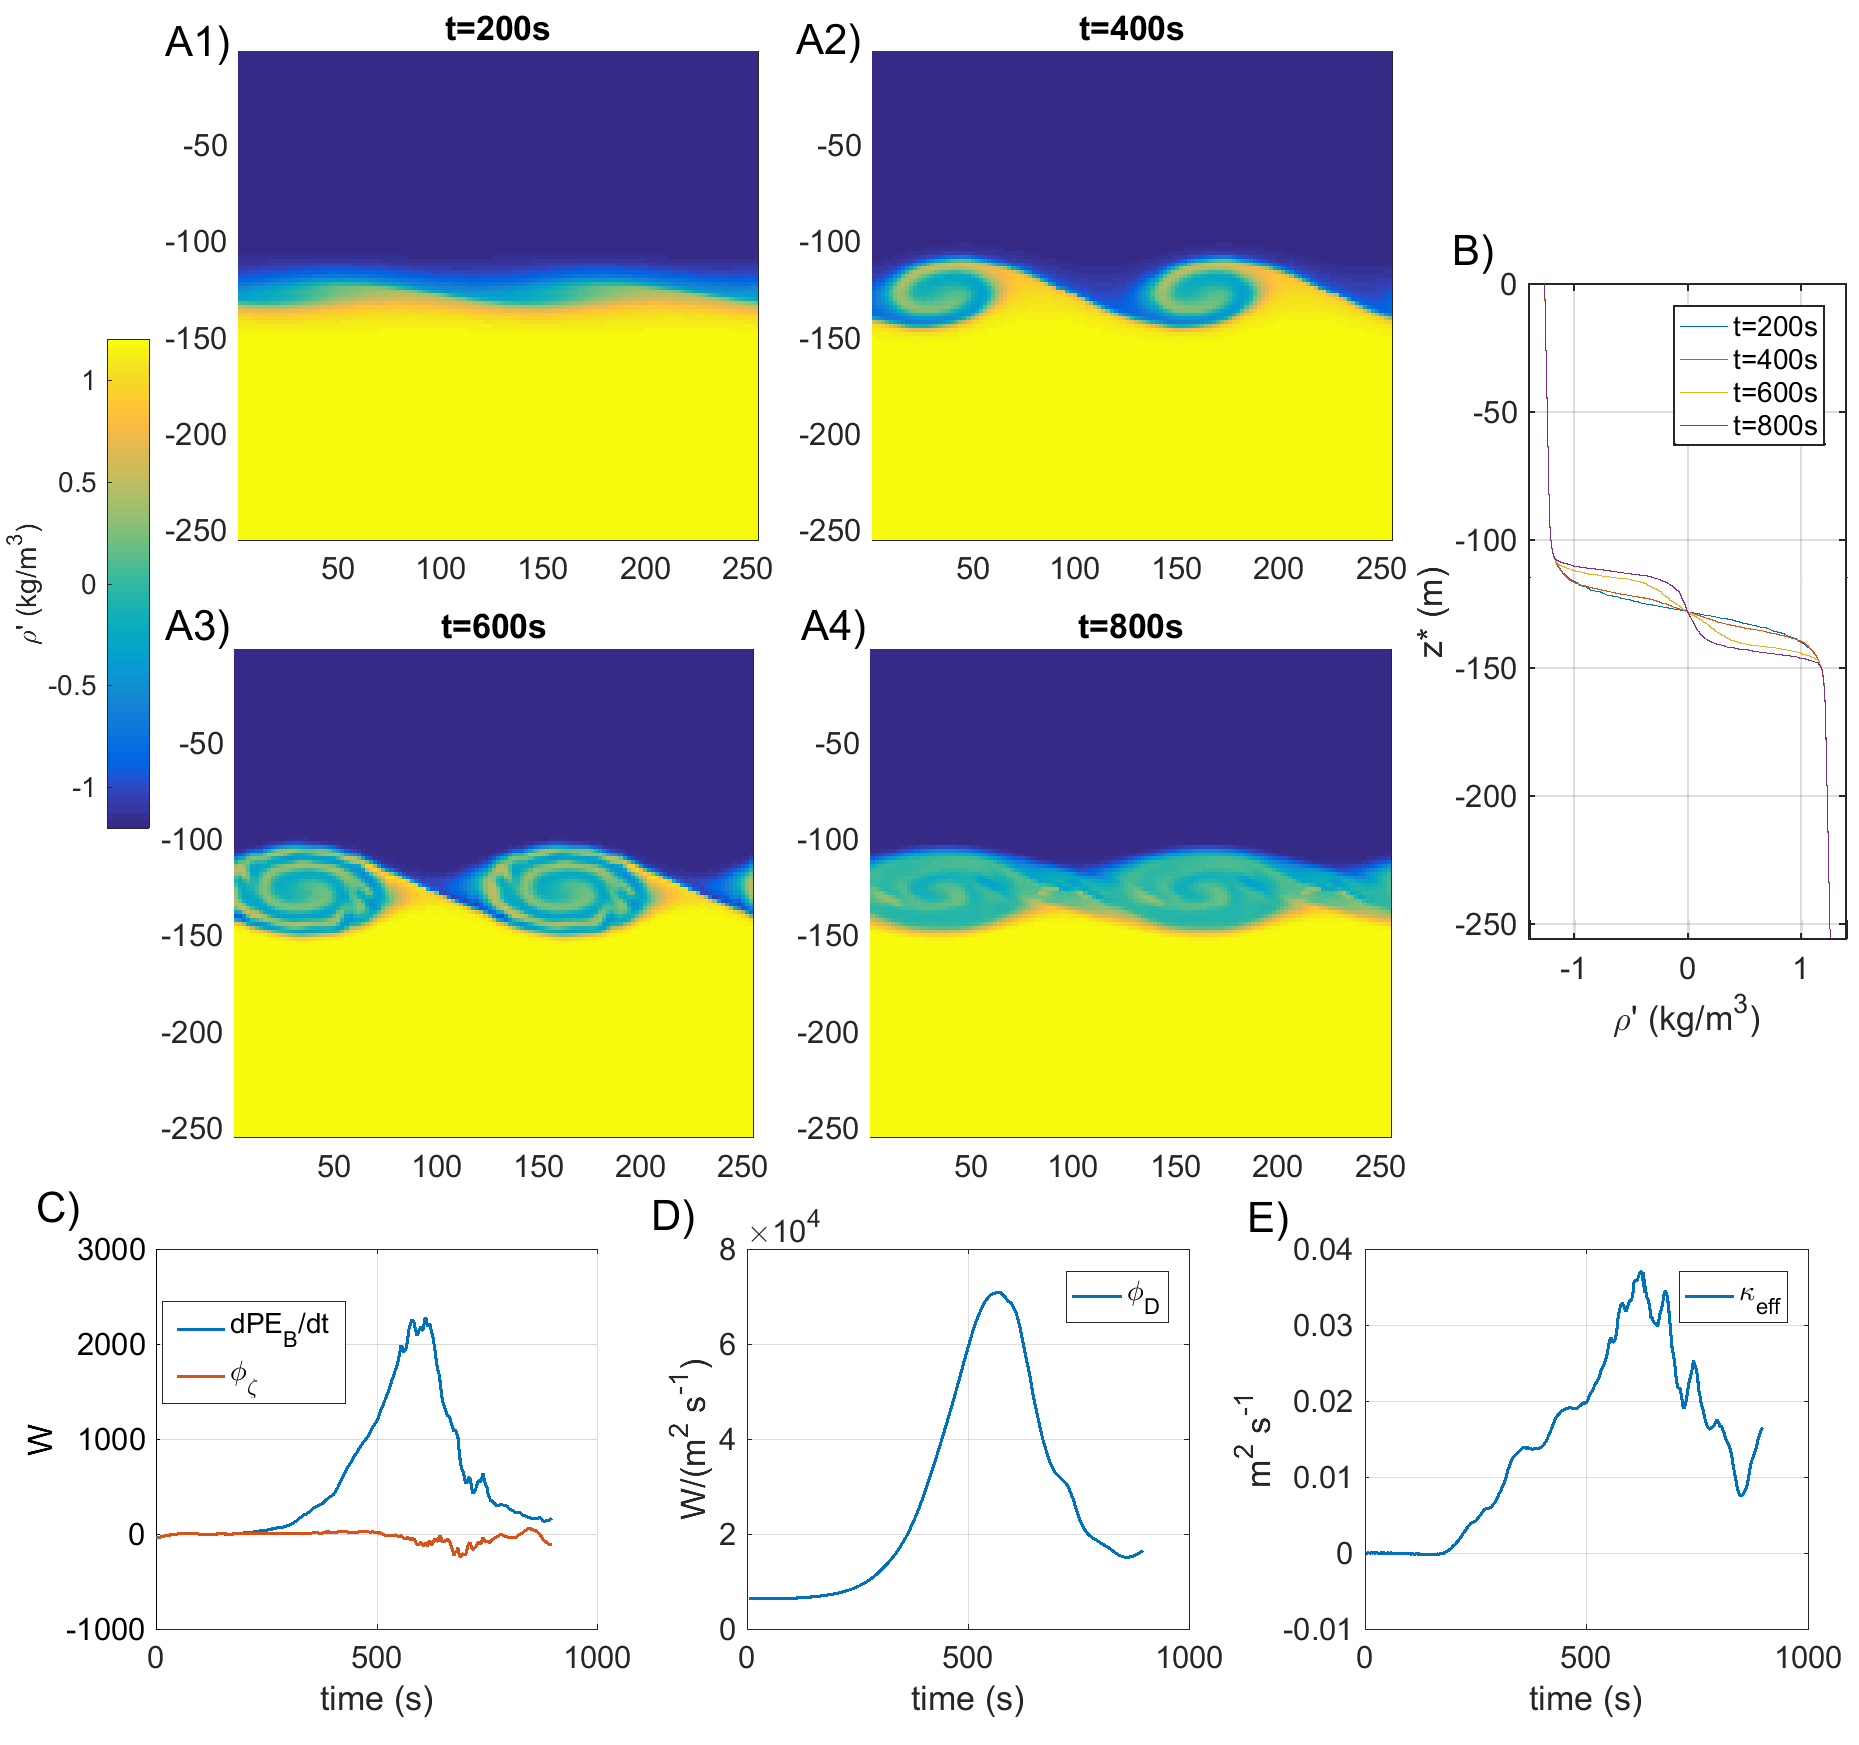
\includegraphics[width=1\textwidth]{./CHAP_BPE/Fig_KH2.png}
\caption{KH testcase}
\label{figCkh}
\end{figure}

\begin{itemize}
\item dx$=$dz$=$2m,$\rho_0 = 1034kg/m^3$ ,amplitude cisaillement courant initial 2m/s, cyclic in x, free surface, based on experiments of \citet{penney_2020}.
\item In this domain develop two billows.
\item fig (\noparref{figCkh}.A1) to (A4) show evolution of field of $\rho$ at $t=200s,400s,600s,800s$, figure (\noparref{figCkh}.B) gives evolution of reference profile at those same times. Figures of lower row give term for balance. Here $\phi_{\zeta}$ is not too important, see in computation of $\kappa_{eff}$ start increasing after $t=200s$ as billows develop, reaches a maximal value at $t=600s$ which coincide whith maximum of $\phi_D$ (higher gradient of density).
\item Once instability has mixed, in reference profile see development of an intermediate homogenous layer between $z*=110m$ and $140m$, coincides with a lowering of $\kappa_{eff}$.
\end{itemize}

%%%%%%%%%%%%%%%%%%%%%%%%%%%%%%%%%%%%%%%%%%%%%
\subsection{CROCO experiments : GBR2D}
\begin{figure}[h!]
\centering
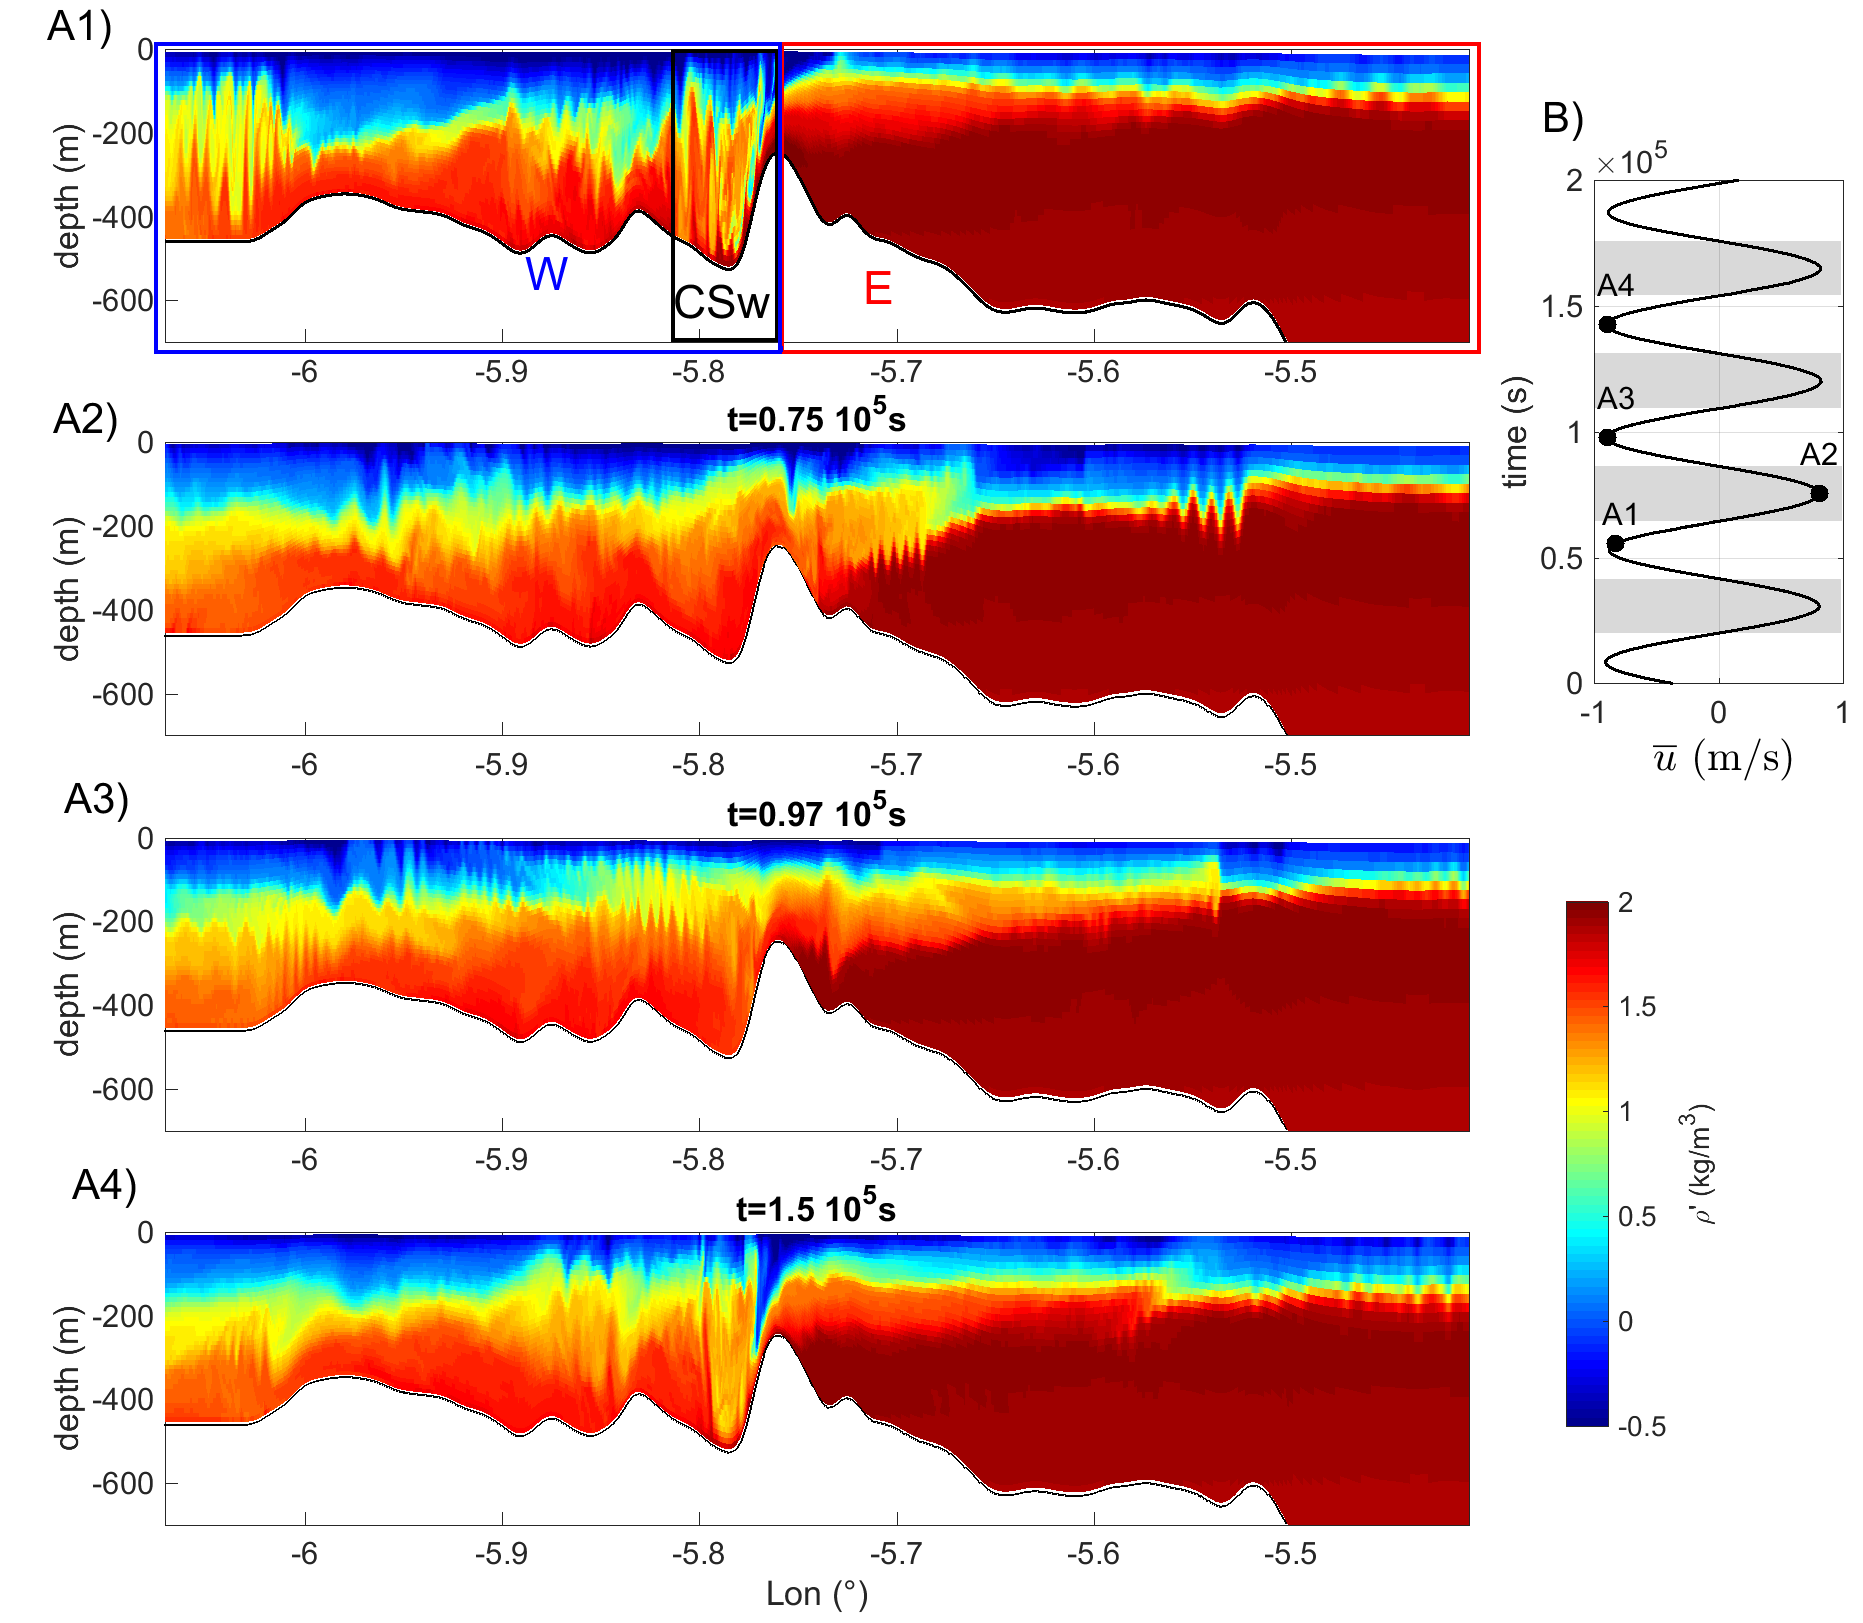
\includegraphics[width=1\textwidth]{./CHAP_BPE/Fig_Kappa_CS_ex.png}
\caption{Definition of domain and snapshots}
\label{figCgbr2d_ex}
\end{figure}

\begin{figure}[h!]
\centering
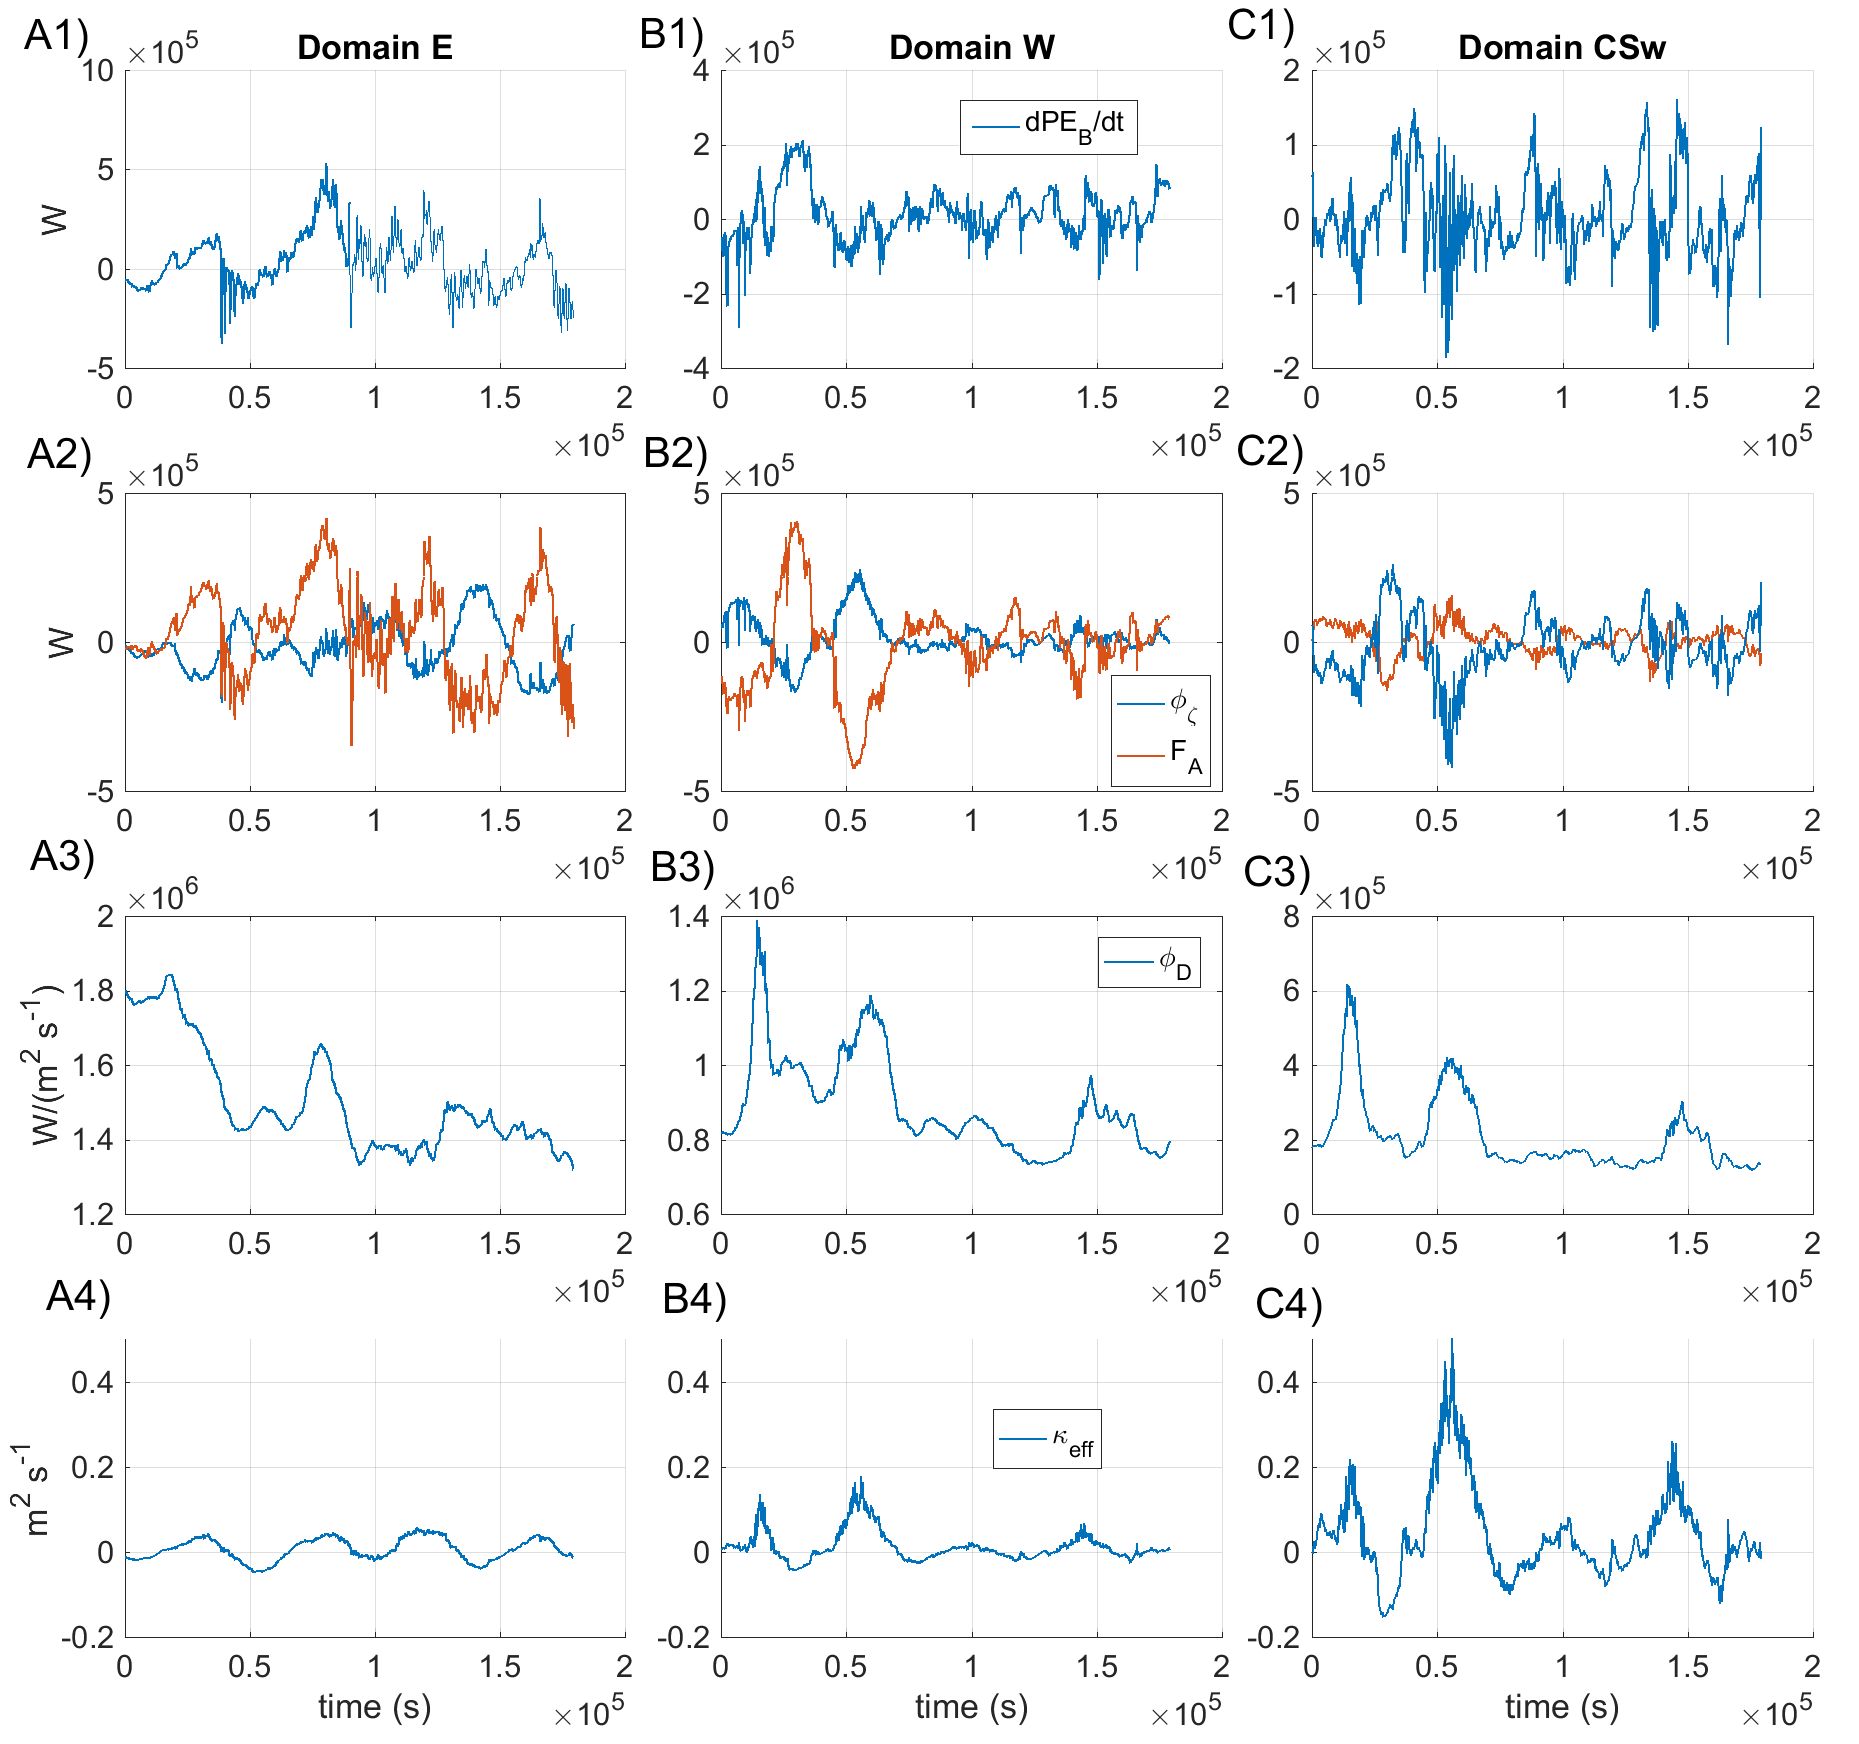
\includegraphics[width=1\textwidth]{./CHAP_BPE/Fig_Kappa_CS.png}
\caption{In each domain}
\label{figCgbr2d}
\end{figure}
\begin{itemize}
\item Based on simulation \textbf{SimRef} of chapter \ref{chapGBR2D}. Here $t=0s$ is at simulation time $6.29T$ at beginning of the first outflow after the spin-up period, and end is $t=10.3T$ with $T=12.4H$ the period of semi-dirunal tide
\item BPE analysis over some of the domain as shown in figure \ref{Fig_Kappa_CS_ex}. \color{red}$\rho_0=$\color{black}
\item Figure \ref{figCgbr2d} gives the evaluation of $\kappa_{eff}$ for each domain, along with term of the balance of equation XXX . 
\item The evolution of $dPE_B/dt$ is a noisy signal that is largely explained by the sum of the non-diffusive terms $F_a$ and $\phi_{\zeta}$, those two terms have the same order/importance
\item Diffusive flux through the boundaries is negligible against$\phi_D$ 
\item When evaluate $\kappa_{eff}$, find a temporal evolution that is not as noisy. For the east part of the domain (E), see an almost sinusoidal signal of period $T$ that correlates with evolution of barotropic currents (positive when $|u|$ positive...)
\item For the west domain (W) and its subdivision (CSw and CSww), this $T$ periodicity is still apparent, not as regular oscillations but as intermitent episodes of higher (positive) $\kappa_{eff}$ during outflows (when $|u|<0$).
\end{itemize}


\subsection{Conclusion}

\begin{itemize}
\item $\kappa_h=\kappa_v=\kappa$ not correct if use this method to evaluate implicit numerical diffusion of advection scheme : implicit diffusion added along the advection direction (not isotropic diffusion).
\item Due to reference profile $z^*$ being local, in two consecutive domains, the boundary fluxes exiting one are not equal to the one entering the other. 
\item The RHS terms of the balance of equation \ref{bilanBPEal} must explain the evolution of the quantity $PE_B$. In an open domain with free surface, advection and movement of this free surface will make $PE_B=\iiint_V \rho g z^* d\tau$ evolve as can be expected through change in the composition of the mass field (through $F_a$) and of the volume (through $\phi_{zeta}$). In most cases here, those two terms are of the same order and are the largest contribution to $dPE_B/dt$.
\item $\kappa_{eff}$ is found to complete the balance once those two contributions are taken into account and is supposed to reflect diapycnal mixing. Here however can see that often find . In open boundary cases especially will have time-evolution appear.
\item $\kappa_{eff}$ as an instantantaneous, homogeneous, isotropic quantity.... but mixing can be seen plutôt comme gradual process?
\item Computation made offline, when evaluate for open-boundary have to be careful in sampling frequency...
\end{itemize}

